\documentclass[a4paper, 10pt]{article}
\usepackage[utf8]{inputenc}
\usepackage[protrusion=true, expansion=true]{microtype}
\usepackage[hang, small, labelfont=bf, up, textfont=it, up]{caption}
\usepackage{graphicx}
\usepackage{fancyhdr}
\usepackage[a4paper, total={7in, 10in}]{geometry}
\usepackage[ddmmyyyy]{datetime}
\usepackage{lipsum}

\pagestyle{fancy}

\lhead{}
\chead{}
\rhead{}

\lfoot{Relatório de Apresentação}
\cfoot{}
\rfoot{\footnotesize Folha \thepage\ }

\renewcommand{\headrulewidth}{0.0pt}
\renewcommand{\footrulewidth}{0.3pt}

%opening
\title{Relatório de Apresentação}
\author{Daniel Bailo}

\begin{document}

\maketitle

\section{Introdução}
\lipsum[1]

\section{Sobre os Dados}
\lipsum[2]

\newpage

\section{Dados Estatísticos}

Algum texto aqui, explicação dos dados por exemplo...\\
Mínimo: 10.72: Magreza grave\\
Máximo: 50.34: Obesidade Grau III(mórbida)\\
Diferença entre o Máximo e o Mínimo: 39.61: Obesidade Grau II(severa)\\
Média: 26.04: Sobrepeso\\
Média por Força: 26.47: Sobrepeso\\
Média Aritmética: 26.47: Sobrepeso\\
Desvio Padrão: 9.11\\
Variância: 83.09

\subsection{Percentil}

Algum texto aqui, explicação do percentil por exemplo...\\
IMC Médio do 1º Percentil: 15.62: Magreza grave\\
IMC Médio do 2º Percentil: 21.51: Saudável\\
IMC Médio do 3º Percentil: 28.21: Sobrepeso\\
IMC Médio do 4º Percentil: 37.89: Obesidade Grau II(severa)\\

\begin{center}
	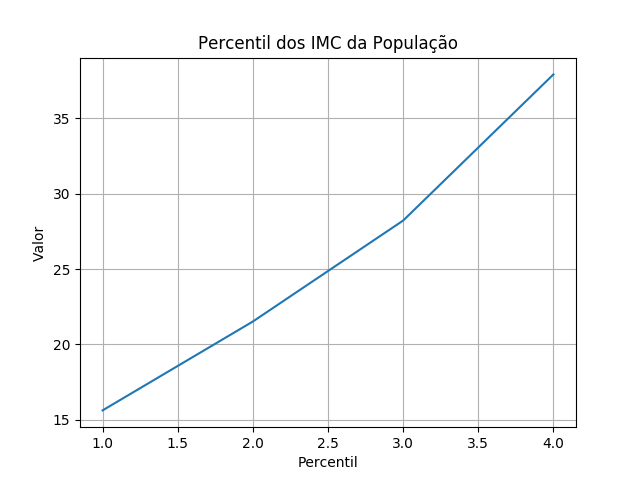
\includegraphics[width=0.8\textwidth]{percentil.png}
	
\end{center}

\section{Conclusão}
\lipsum[3]

\end{document}
